\documentclass[14pt, a4paper]{extarticle}
\usepackage{fefu_title}

\titlelabel{\thetitle.\quad}

\graphicspath{{./}}
\DeclareGraphicsExtensions{.png, .jpg}

\renewcommand{\cftsecleader}{\cftdotfill{\cftdotsep}}
\let \savenumberline \numberline
\def \numberline#1{\savenumberline{#1.}}

\counterwithin*{equation}{section}

\lstset{
	basicstyle=\fontsize{12}{12}\selectfont\ttfamily
}

\begin{document}
	\fefutitlepage{Б8118-02.03.01сцт}{Мышалов Р.Е.}{7}{июня}{2020}
	
	\tableofcontents
	\pagebreak
	
	\section{Введение}
		В данной лабораторной работе нам предстоит покайфовать с диффурами
		\pagebreak
		
	\section{Для следующих линейных дифференциальных уравнений дать характеристику и найти общее решение}
		\begin{enumerate}
			\item \(y'' +4y = 0\)
			
				Характеристика: уравнение второго порядка, не содержит независимого аргумента и первой производной функции
				
				Общее решение: \(y (x) = C_2\sin{(2x)} + C_1\cos{(2x)}\)
				
			\item \(y'' + 2y' + 5y = 5x \cdot e^{-x} \cdot  \sin{2x}\)
			
				Характеристика: уравнение второго порядка с постоянными коэффициентами
			
				Общее решение: \[y (x) = e^{-x} \left(C_1\sin{(2x)} + C_2\cos{(2x)} - \dfrac{5}{8} \cdot x^2 \cos{(2x)} + \dfrac{5}{16} \cdot x \sin{(2x)}\right)\]
				
			\item \(y'' - \dfrac{3}{x} \cdot y' + \dfrac{6}{x^2} \cdot y = 0\)
			
				Характеристика: уравнение второго порядка с переменным коэффициентами
			
				Общее решение: \(y(x) = C_1 \cdot x^2 \sin{(\sqrt{2} \ln{x})} + C_2 \cdot x^2 \cos{(\sqrt{2} \ln{x})}\)
				
			\item \(y'' - \dfrac{y'}{x} + \dfrac{y}{x^2} = 0\)
			
				Характеристика: уравнение второго порядка с переменным коэффициентами
			
				Общее решение: \(y(x) = C_1 \cdot x + C_2 \cdot x \ln{x}\)
				
			\item \(y'' - \dfrac{y'}{x} + \dfrac{y}{x^2} = 0\)
			
				Характеристика: уравнение третьего порядка с переменным коэффициентами
			
				Общее решение: \(y(x) = \dfrac{C_1}{x^3} + \dfrac{C_2}{x^2} + C_3 + \dfrac{\ln^2{x}}{12} - \dfrac{5\ln{x}}{36}\)
		\end{enumerate}
		\pagebreak
			
	\section{Для заданных уравнений найти решение, удовлетворяющее заданным условиям, построить его график}
		\begin{enumerate}
			\item \(x^4 y'' + \left(xy' - y\right)^3 = 0; \qquad y(1) = 0, \quad y'(1) = 2i\)
		\end{enumerate}
		\pagebreak
		
	\section{Для модели «Хищник-Жертва» описать поведение решений соответствующих уравнений системы при заданных коэффициентах, построив график решения}
		\begin{align*}
			\begin{cases}
				\dfrac{dx}{dt} = \left(\alpha - \beta \cdot y\right) \cdot x \\ \\				
				\dfrac{dy}{dt} = \left(\delta \cdot x - \gamma \right) \cdot y
			\end{cases}
			\parbox{100pt}{\(\alpha = \gamma = 0.29\)  \\ \(\beta = \delta = 0.29\)}
			x(0) = y(0) = 1
		\end{align*}
		\hspace{1cm}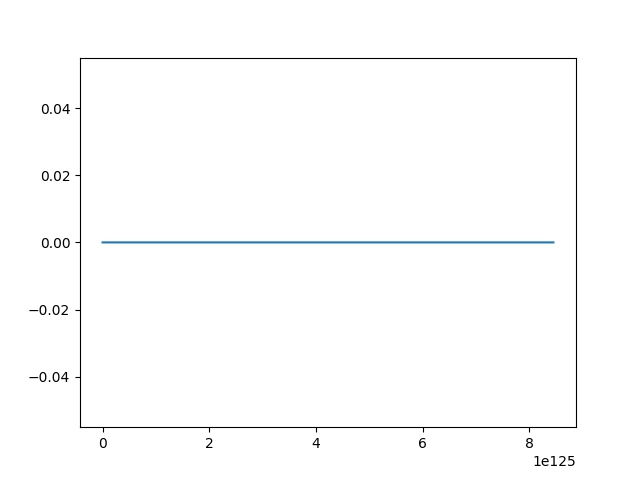
\includegraphics[width=15cm]{plot}
		\pagebreak
		
		\begin{lstlisting}[language=Python, frame=single, gobble=5, tabsize=2]
			import matplotlib.pyplot as plt
			
			def get_x(x, y, alpha, beta):
				return (alpha - beta * y) * x
			
			def get_y(x, y, delta, gamma):
				return (delta * x - gamma) * y
			
			def get_data(x, y, alpha, beta, delta, gamma, step):
				data = [[], []]
				for i in range(0, 1000000):
					data[0].append(get_x(x, y, alpha, beta) * step + x)
					data[1].append(get_y(x, y, delta, gamma) * step + y)
					x = data[0][i]
					y = data[1][i]
				return data
			
			def main():
				y = 0
				x = 1
				step = 0.001
				alpha = gamma = 0.29
				beta = delta = 0.29
			
				data = get_data(x, y, alpha, beta, delta, gamma, step)
			
				plt.plot(data[0], data[1])
				plt.savefig('plot.png')
				plt.close()
			
			if __name__ == "__main__":
				main()
			
		\end{lstlisting}
		
\end{document}